\title{Generating Fugal Sequences with Clojure, Occam and Reconstructability Analysis}
\author{Ryan Spangler}
\date{\today}

\documentclass[11pt]{article}

\usepackage{commath}
\usepackage{graphicx}
\usepackage{listings}
\usepackage{amsfonts}

% python highlighting ----------
\usepackage{color}
\usepackage{listings}
\usepackage{textcomp}
\usepackage{setspace}
\usepackage{hyperref}
%\usepackage{palatino}

%\doublespacing

\setcounter{secnumdepth}{0}

\begin{document}
\maketitle

\section{Introduction}

I have long suspected that Bach's fugues have a high degree of internal relatedness, though I have never had the tools to quantify that until now.  This project is a journey to define just how internally related Bach's fugues are, using the means at my disposal (namely Occam and Clojure, along with the theory behind RA).  It is an attempt to not just analyze, but also to generate new fugues using the form of old ones.  Given the scores of Bach's fugues (48 in all), I tease apart the separate lines into sequences of notes and use these sequences to form predictions about what the next note is, given a series of previous notes.  Applying these predictions iteratively to a seed note generates new sequences of notes, which can then be layered and played back.  Two supporting Clojure libraries have sprung from this project, \href{http://github.com/prismofeverything/occam}{occam} (the clojure version!) and \href{http://github.com/prismofeverything/fuga}{fuga}.  These are open source projects anyone can use to analyze midi files and generate fugues of their own, which I discuss in the next section.  

Bach fugues are each unique, but have a similar overall structural philosophy.  They each start with a single voice which lays out a theme, and is ultimately joined by a series of voices each performing variations on the original.  Each line gets superimposed over the others, and part of the challenge of writing a fugue is tying these lines together in a meaningful and harmonious way (of which Bach is the generally acknowledged Khan of this arena).  In order to predict sequences, the common structures and gestures that thematically tie the fugue together have to be extracted and applied on new sequences.  Part of the symmetry of the fugal lines is that the theme is repeated, but in a different key or mode.  In this way, the information in contained in a relative, rather than an absolute way, and the analysis of the notes data has to reflect this relativity.

\section{Methods}

The process of generating new note sequences given a set of existing note sequences takes many steps.  First, the note files are parsed and the notes are extracted into a simple key based data format containing a field for the tone, the begin time and the end time.  In this form many notes could be happening at once, representing the separate voices of the fugue playing in polyphony.  In addition, the onset times are not exactly simultaneous, but fluctuate around a mean with epsilon < 10 time steps.  So all notes are grouped into simultaneous occurances and these groups are sorted by their mutual onset.  Then, separate lines are drawn out of these groups by stepping through each coinciding time step and finding a previous and subsequent note from the previous and subsequent group for each note in that time step.  This step is not perfect and note jumps of more than 10 are excluded (arbitrarily, but better to assume too little!)  This reduces the series of notes into a handful of chains.  

Once the chains are in hand, they can be reduced to a series of snapshots of fixed length relative gestures.  This length is variable, so that a variety of lengths can be explored for predictionary power.  One of the main uses of Occam in this project was to discover how many previous notes should be taken into account to predict the next note.  I explored up to 5, where the defining the data would require two more notes than I wanted to use when doing the prediction.  Given a chain of notes $[61 63 66 63 61 64 68]$ (where 60 is middle C) this can be pivoted on the second to last note (in this case the 64) and all of the previous notes can be masked relative to that one, resulting in $[-3 -1 +2 -1 -3 0 +4]$.  The values leading up to the 0 are the previous notes in the chain, the 0 represents the value of the note we will be making the prediction for, and the last value is the dependent variable, the relative shift of the note given what notes came before it.  That way 7 notes can be used as a case for 5 previous notes predicting the subsequenct note given the current one.

All the chains are reduced to rows in the above relative format by passing a window over them, taking each seven values one after the other.  This is written out to Occam format and fed into the Occam web console.  In the above case, the independent variables are represented as ABCDE and the dependent variable is Z.  We don't need to the pivot note itself because it is always zero by definition:  all other notes are considered relative to it for this row.  This is the results matrix for five previous predicting notes A-E:

\begin{center}
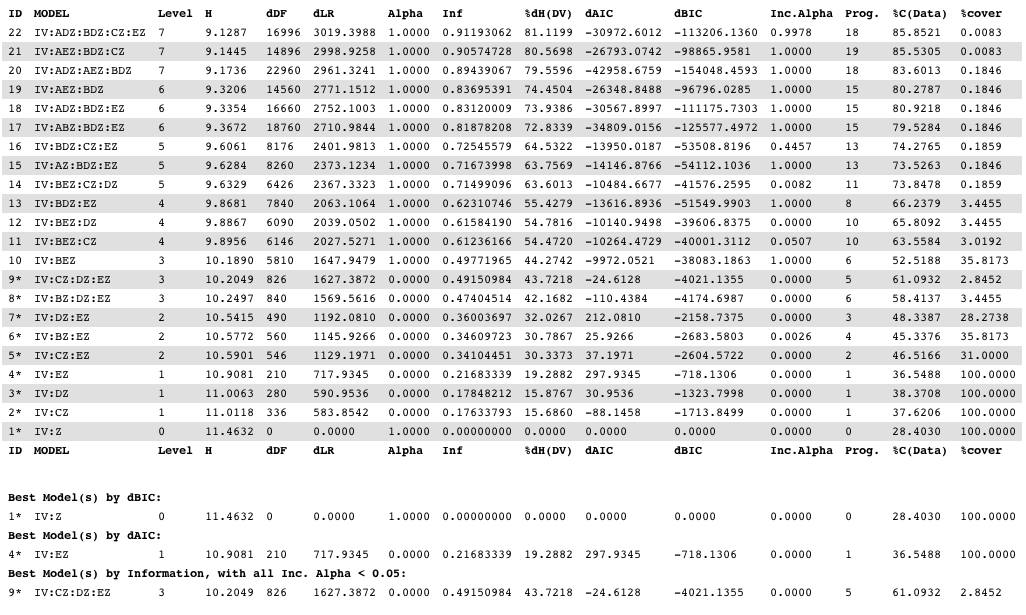
\includegraphics[scale=0.45]{five.png}
\end{center}

From this table, the best model by information is CZ:DZ:EZ!  This is the point just before alpha flips to 1.0 from 0.0.  Also, this precedes a huge jump in dDF, which strikes a balance between simplicity and power.  Which means that only three previous notes need to be tracked to reasonably predict the next note, not all five.  

I take this to heart and run a fit on a series of three note predictions AZ:BZ:CZ.  The fit table is too large to print here, but can be found in the \href{http://github.com/prismofeverything/fuga}{fuga} repository under occam/fit/*.  This shows all the combinations of probabilities for each independent variable.  These all have a cardinality somewhere between 16 and 30, depending on how many relative jumps were really observed.  The dependent variable for this run has 15 observed states.  

The next step is parsing these fit tables into trees whose path for each row is given by the states of all the independent variables and whose value at that node is all of the possible outcomes and their relative probabilities.  If nothing is found for that path, a shorter path is used on a similar tree created from data with only two previous notes (and therefore TWO independent variables).  If this again is not found, a third tree built on the data for a single previous note is used, which is always found.  Then, given a seed path (which can even be a single note), this process can be iterated, casting the three previous notes relative to the latest note and using this as a path into the probability tree, where the resulting state is found from choosing from the possible outcomes weighted by their relative probabilities.  This gives an arbitrarily long sequence of notes, which can then be recast into note events and passed on to the midi output player.  

\section{Results}

\section{Discussion}

\section{Conclusion}

\end{document}

